% The submission document. build_check.tex stays as the fast chapter-only compile; this is
% the one that carries the front matter, the numbering and the format the university wants.
\documentclass[12pt,a4paper]{report}

\usepackage[utf8]{inputenc}
\usepackage[T1]{fontenc}
\usepackage{mathpazo}
\usepackage[margin=1in,left=1.5in]{geometry}
\usepackage{setspace}
\usepackage{amsmath}
\usepackage{booktabs}
\usepackage{enumitem}
\usepackage{graphicx}
\usepackage{array}
\usepackage{fancyhdr}
\usepackage[hidelinks]{hyperref}

% Binding edge takes the wider margin; 1.5 line spacing is the usual requirement for a
% submitted dissertation and leaves room for an examiner's annotations.
\setstretch{1.5}

\pagestyle{fancy}
\fancyhf{}
\fancyhead[L]{\footnotesize\textit{B.Sc.\ Physics -- Dissertation}}
\fancyhead[R]{\footnotesize\textit{Brian Mwai -- 1050555}}
\fancyfoot[C]{\thepage}
\renewcommand{\headrulewidth}{0.4pt}

\begin{document}

% Front matter for the dissertation. The title page follows the format used in the approved
% research proposal (Research_Proposal_Brian_Mwai_v2.tex); the declaration, abstract and
% front lists are added because a dissertation requires them and the proposal had none.

\begin{titlepage}
\centering
{\setstretch{1.0}
\vspace*{0.4cm}


\includegraphics[height=3.2cm]{assets/cuea.png}

\vspace{0.7cm}

{\Large\bfseries THE CATHOLIC UNIVERSITY OF EASTERN AFRICA}

\vspace{0.3cm}
{\large Faculty of Science}

\vspace{0.2cm}
{\normalsize Department of Natural Sciences}

\vspace{1.6cm}

{\LARGE\bfseries\scshape Dissertation}

\vspace{1.0cm}

{\Large\bfseries A Cortical-Proxy Observable for\\[6pt]
Emotionally Manipulative Media:\\[6pt]
An Instrument, a 400-Item Corpus,\\[4pt]
and a Field Bound}

\vspace{1.8cm}

\begin{tabular}{r l}
\textbf{Student Name:}      & Brian Mwai \\[5pt]
\textbf{Admission Number:}  & 1050555 \\[5pt]
\textbf{Programme:}         & Bachelor of Science in Physics \\[5pt]
\textbf{Supervisor:}        & Dr.\ Songa Mutambi \\[5pt]
\textbf{Date:}              & \today \\
\end{tabular}

\vfill

{\small A dissertation submitted in partial fulfillment of the requirements\\
for the degree of Bachelor of Science in Physics.}

\vspace{0.8cm}
\par}
\end{titlepage}

\pagenumbering{roman}
\setcounter{page}{2}
% Front matter carries no running head: there is no chapter or section for one to name, and a
% stale mark left over from the title page is worse than none.
\pagestyle{plain}

\chapter*{Declaration}
\addcontentsline{toc}{chapter}{Declaration}

This dissertation is my own original work and has not been presented for the award of a
degree at this or any other university. The instrument, the corpus, the analysis scripts and
the text are mine. Where the work of others is used it is cited, and the released model
checkpoint, the public datasets and the software libraries the work builds on are named in
the chapters that use them.

No part of the measurement or the analysis was contributed by any person other than the
author. The supervision named below was academic guidance and approval, not authorship.

\vspace{0.9cm}

{\setstretch{1.0}
\noindent\begin{tabular}{@{}p{0.42\textwidth}@{\hspace{0.08\textwidth}}p{0.42\textwidth}@{}}
\textbf{Brian Mwai} & \\
Admission Number 1050555 & \\[1.1cm]
\hrule\vspace{4pt} Signature & \hrule\vspace{4pt} Date \\
\end{tabular}

\vspace{1.0cm}

\noindent This dissertation has been submitted for examination with my approval as the
university supervisor.

\vspace{0.9cm}

\noindent\begin{tabular}{@{}p{0.42\textwidth}@{\hspace{0.08\textwidth}}p{0.42\textwidth}@{}}
\textbf{Dr.\ Songa Mutambi} & \\
Department of Natural Sciences, Faculty of Science & \\
The Catholic University of Eastern Africa & \\[1.1cm]
\hrule\vspace{4pt} Signature & \hrule\vspace{4pt} Date \\
\end{tabular}
\par}

\chapter*{Abstract}
\addcontentsline{toc}{chapter}{Abstract}

Media is routinely modelled in statistical physics as an external field acting on a
population of coupled opinion states, and that field is almost never measured. This
dissertation builds an instrument that measures a candidate observable from content itself,
applies it to a corpus, and reports what the measurement can and cannot support.

The observable is a cortical proxy. Text is spoken, transcribed, embedded, and passed to
TRIBE v2, a released encoder that predicts cortical response; two networks are averaged from
that prediction, one associated with affective salience and one with deliberative control,
and the index is their signed difference. The ratio form specified in the proposal is
undefined for $17.25\%$ of items and was replaced by that difference. Nothing here is a
measurement of a person: no participant was scanned, and the observable is never identified
with any subcortical structure.

A corpus of 400 items across four categories, matched on length, was scanned on a GPU. The
categories separate at $\eta^2 = 0.1068$, $F = 15.779$, $p = 1.035\times10^{-9}$, against a
design powered to detect $\eta^2 = 0.0268$, and the index discriminates the pre-scan
manipulative label at $\mathrm{AUC} = 0.6274$. The separation is carried almost entirely by
fear-activating content, $d = 0.9389$ against neutral, while high-outrage content does not
separate at all, $d = 0.0300$, though it is the category the proposal expected to separate
most. Each category is drawn from a single source dataset, so the separation is between
corpora and cannot be attributed to framing rather than provenance; this confound is stated
before the result wherever the result appears. A second scanning session over all 400 items
gives test-retest $\mathrm{ICC} = 0.8725$ and replicates the separation at $\eta^2 = 0.0888$,
while $12.8\%$ of individual items reverse direction between sessions, so the instrument supports
category-level claims and no per-item verdict is made.

The physics is a mean-field treatment in which media enters as a field $h = \alpha X$ on the
measured observable. Calibrating $\alpha$ against the corpus does not identify it: the fit
performs worse than the sample mean out of sample and the estimate scales with a coupling the
study does not measure, so no value is quoted anywhere. What survives is a necessary
condition, $\alpha \ge h_c(\beta J)/\Delta X$. The measured spread $\Delta X = 0.1241$ gives
$\alpha \ge 4.2938$ at $\beta J = 2$, a constraint on any future proposal of this mechanism
that depends on the range of the observable rather than on why that range arises.

\chapter*{Publications arising from this work}
\addcontentsline{toc}{chapter}{Publications arising from this work}

Three papers were written from this project. All are single-authored by the candidate. Their
status at the time of submission is given as it stands, and no paper is described as
published unless it has been accepted.

\begin{enumerate}
\item \textbf{Bounding the external field in mean-field opinion dynamics: what any content
observable must satisfy to drive a transition.} 12 pages. Prepared for \emph{Physica A}.
Corresponds to Chapter~3, and states the bound $\alpha \ge h_c(\beta J)/\Delta X$ together
with the screening criterion that follows from it. \emph{Status: complete, awaiting
submission.}

\item \textbf{A cortical-proxy observable for emotionally manipulative media: an instrument,
a 400-item corpus, and the field bound it yields.} 12 pages. Prepared for \emph{Physica A} as
the companion to the first. Corresponds to Chapters~4 to~6, and supplies the measured spread
that the first paper's inequality consumes. \emph{Status: complete, awaiting submission.}

\item \textbf{What does a released average-subject brain encoder actually predict? A measured
noise ceiling and a replication protocol.} 6 pages. Prepared for \emph{Imaging Neuroscience}.
Reports the inter-subject noise ceiling measured from public data, and the two silent defects
behind a value this project withdrew. \emph{Status: drafted; one prediction pass remains,
which is specified in the paper and marked as not yet run.}
\end{enumerate}

The instrument, the corpus, the analysis scripts and the artifacts every reported number is
read from are public at \url{https://github.com/brn-mwai/monarch}, and the working instrument
runs at \url{https://monarch.brianmwai.com}.

\chapter*{Acknowledgements}
\addcontentsline{toc}{chapter}{Acknowledgements}

I thank my supervisor, Dr.\ Songa Mutambi, for approving a change of instrument mid-project
when the released checkpoint turned out not to see the structure the proposal named, and for
insisting that the reformulated index be defended on its own terms rather than presented as a
minor substitution.

This work runs on public artifacts. TRIBE v2 and its released checkpoint come from Meta AI
Research; the corpus is assembled from ISOT, SemEval-2019 Task 4, Webis-Clickbait-17 and
PubMed; the fMRI recordings used to measure the noise ceiling come from the Algonauts 2025
release. The GPU time came from Kaggle's free tier, and the constraints of that tier shaped
how the corpus was scanned.

\tableofcontents

\listoffigures
\addcontentsline{toc}{chapter}{List of Figures}

\listoftables
\addcontentsline{toc}{chapter}{List of Tables}

\chapter*{Abbreviations and Symbols}
\addcontentsline{toc}{chapter}{Abbreviations and Symbols}

\begin{tabular}{@{}l l@{}}
\textbf{NAA} & Network Activation Asymmetry, the observable this work measures \\
$A_{\text{aff}}$ & Mean predicted activation across affective-salience regions \\
$A_{\text{del}}$ & Mean predicted activation across deliberative-control regions \\
$\mathrm{NAA}_{\text{signed}}$ & $A_{\text{aff}} - A_{\text{del}}$, the signed index used throughout \\
$\Delta X$ & Measured spread of the observable across the corpus \\
$\alpha$ & Coupling between the observable and the model's external field, $h = \alpha X$ \\
$\beta J$ & Reduced interaction coupling in the mean-field model \\
$h_c$ & Critical field at which the mean-field free energy loses bistability \\
$\eta^2$ & Proportion of variance explained, the effect size for category separation \\
AUC & Area under the receiver operating characteristic curve \\
ICC & Intraclass correlation coefficient, absolute-agreement form ICC(2,1) \\
fMRI & Functional magnetic resonance imaging \\
ROI & Region of interest \\
TR & Repetition time, one fMRI sampling interval \\
\end{tabular}

\cleardoublepage
\pagestyle{fancy}
\pagenumbering{arabic}
\setcounter{page}{1}


\chapter{Introduction}
\label{ch:intro}

\section{The problem}

Two articles can report the same event and leave a reader in entirely different states. One
informs; the other provokes. Readers notice the difference and cannot quantify it, and the
platforms that distribute both have no objective measure of which they are amplifying. The
difference is real, consequential and unmeasured.

Existing approaches measure the text. Sentiment analysis counts affective vocabulary;
readability scores count syllables and clause length; stance detection classifies a position.
None of them measures what the content is predicted to \emph{do} to the person reading it.

This project takes a different route. Rather than characterising the words, it estimates the
response: a released neural encoder predicts cortical activity from the content, and the
measurement is taken on that prediction. The instrument is a thermometer for one specific
property of media, and the thesis is an account of building it, running it, and stating
carefully what its readings support.

\section{The amendment, stated at the outset}
\label{sec:amendment}

Three commitments in the original proposal could not be met as written. They are set out here
rather than disclosed in the results chapter, because a reader who meets them for the first
time beside a result will reasonably suspect they were discovered to explain it. Each was
identified before the measurement was taken, and each is documented in the amendment approved
by the supervisor.

\textbf{First, the observable is cortical.} The proposal framed the index around subcortical
affective structures. The released checkpoint predicts cortical surface activity only, over
$20{,}484$ vertices, and contains no subcortical output. The index is therefore a
\emph{cortical proxy}: a contrast between two cortical ROI unions, one associated with
affective salience and one with deliberative control. No claim about subcortical structures
appears anywhere in this document.

\textbf{Second, the index is a difference, not a ratio.} Equation~(4) of the proposal defines
the index as $A_{\mathrm{aff}}/(A_{\mathrm{del}} + \delta)$. The encoder emits standardised
activation, so an ROI mean is negative about as often as positive and the ratio sign-flips or
diverges. On the completed corpus it is undefined for $17.25\%$ of items. The measurement uses
the signed difference $A_{\mathrm{aff}} - A_{\mathrm{del}}$, which is defined everywhere and
is the form the physics requires.

\textbf{Third, the corpus is text-only.} The proposal specified 1{,}500 multimodal items. The
delivered corpus is 400 text items in four balanced categories, and Research Question~IV,
which required audio and video, is out of scope.

\section{Research questions}

\begin{description}
\item[RQ I] Can predicted cortical activation serve as a quantitative signature of
emotionally manipulative media content, and how does the resulting index perform as a
classifier against human labels?

\item[RQ II] How is the index distributed across content categories, and do the categories
separate?

\item[RQ III] What phase structure does a mean-field opinion model exhibit under a field
derived from this observable, and what does the measured spread imply for the coupling?

\item[RQ IV] How do text, audio and video contribute to the index? \emph{Out of scope under
the amendment.}
\end{description}

\section{Objectives}

\begin{enumerate}[label=(\roman*)]
\item Build a labelled corpus of media items in balanced categories.
\item Run the encoder over the corpus and compute the index for every item.
\item Characterise the distribution of the index.
\item Calibrate the coupling between the index and the model's field.
\item Derive the phase structure of the opinion model.
\item Validate the index as a classifier against human labels.
\item Deliver the measurement apparatus as working open-source code.
\end{enumerate}

Objective (vii) is the primary deliverable. The proposal states this explicitly and it governs
how the work should be assessed: the apparatus is the promise, and the empirical result is
what the apparatus returned when it was run.

\section{Contribution}

Three, developed across the chapters that follow.

A \textbf{bound} on the coupling between any content observable and an opinion-dynamics field,
requiring only the observable's measured spread and the model's own spinodal, and evaluable
before data are collected (Chapter~3).

An \textbf{instrument}, delivered as open-source code, together with the documented finding
that the released checkpoint is cortical-only and that its agreement with real cortex is
contested (Chapter~4).

A \textbf{measurement} over 400 items, reported with the design's sensitivity attached and its
central confound stated before its interpretation (Chapters~5 and~6).

\section{Structure of this document}

Chapter~2 reviews the literature on opinion dynamics as statistical physics and on predictive
neural encoding, and identifies the gap this work addresses. Chapter~3 derives the
theoretical framework and the bound. Chapter~4 describes the instrument, the corpus and the
analysis. Chapter~5 reports the results. Chapter~6 discusses what they support. Chapter~7
concludes.

\chapter{Literature Review}
\label{ch:literature}

This work sits between two literatures that rarely meet: the statistical physics of opinion
dynamics, which supplies the model, and predictive neural encoding, which supplies the
observable. The gap it addresses lies precisely at their junction.

\section{Opinion dynamics as statistical physics}

The programme of treating collective opinion with the tools of statistical mechanics is
established and productive. Castellano, Fortunato and Loreto's review \cite{castellano2009}
remains the standard survey: binary attitudes map to Ising spins, social conformity to a
ferromagnetic coupling $J$, and external influence to a field $h$. Galam's review of his own
models \cite{galam2008} traces the same lineage through majority-rule dynamics, and
Sznajd-Weron and Sznajd \cite{sznajd2000} contribute the outward-influence variant that
carries their name. Stauffer \cite{stauffer2008} gives an accessible account of why
two-dimensional Ising models apply to social questions at all.

The recent review by Mullick and Sen \cite{mullick2025} surveys a century of Ising-inspired
sociophysics across opinion dynamics, markets, segregation and language. Notably for this
work, it lists data-driven calibration against large-scale social datasets among the field's
\emph{open directions} rather than among its accomplishments.

\subsection{How the external field is treated}

Where these models represent media explicitly, the field is assigned rather than measured.
Crokidakis \cite{crokidakis2012} introduces mass media into the two-dimensional Sznajd model
as a probability $p$ of following the media opinion, sweeps it, and finds the phase transition
absent above $p \approx 0.18$. Azhari and Muslim \cite{azhari2023} apply an external field to
majority-rule and $q$-voter dynamics on the complete graph and sweep its magnitude. Freitas,
Vieira and Anteneodo \cite{freitas2020} study imperfect bifurcations and cusp catastrophes
under external bias, parameterised by sensitivity and direction rather than by any measured
quantity. The review of models with external effects by S\^{i}rbu and colleagues
\cite{sirbu2016} surveys this class without any of them measuring the external term.

In each case the swept parameter is the quantity whose real-world magnitude is at issue. The
literature can therefore demonstrate that a population tips at some $h^\ast$ without
establishing that any real influence attains it.

\subsection{The exception, and what it leaves open}

One recent study breaks the pattern. Korbel, Dahdoul and Thurner \cite{korbel2026} calibrate a
double random-field Ising model of elections directly to campaign expenditure and extract a
critical spending threshold from historical results, reporting it as the first time
thermodynamic parameters and a critical threshold have been taken from election data in this
way.

Two things remain open after it, and they define the gap this work addresses. Their
calibration is fitted from outcome data after the fact, so it cannot screen a proposed
mechanism before data exist. And it is specific to expenditure, whereas observables proposed
for media \emph{content} remain uncalibrated. What is missing in both cases is a necessary
condition stated on the coupling itself, which is what Chapter~3 supplies.

\section{Predictive neural encoding}

The second literature concerns models that predict brain responses to naturalistic stimuli.
The relevant instrument here is TRIBE \cite{tribe2025}, a trimodal encoder that combines
pretrained text, audio and video representations to predict fMRI responses to film, trained on
the Courtois NeuroMod recordings and evaluated over 1{,}000 cortical parcels.

Such models make a measurement possible that was not before: rather than characterising a
stimulus by its surface features, one can estimate the response it is predicted to elicit.
That is the move this project makes.

\subsection{What a released checkpoint does and does not guarantee}

A technical report describes an architecture and a training procedure. The weights released
under its name are a separate artifact, and their properties must be established from the
artifact itself.

Three such properties matter here and none is visible from the publication. The checkpoint
used in this work predicts cortical surface activity only. Its loader forces an
average-subject configuration at load time, so per-subject variation is unavailable. And its
agreement with real cortex in that configuration is contested: a commercially published audit
reports vertex-level anti-correlation against a measured inter-subject ceiling, across four
subjects and all seven Yeo networks. That audit is self-published by a company selling the
per-subject alternative, uses one stimulus, and reports small magnitudes in either direction;
it has not been independently replicated. It should be neither accepted uncritically nor
dismissed.

\section{The gap}

Placing the two literatures beside one another gives the gap directly.

The sociophysics literature has a field it cannot measure. The encoding literature has a
predicted response that has not been used as a field. Neither has stated what a candidate
observable would have to satisfy for the mechanism to operate at all.

This work supplies that condition, builds an instrument that produces a candidate observable,
measures its spread on a controlled corpus, and reports what follows --- including the
respects in which the design cannot support the interpretation one would prefer.

\chapter{Theoretical Framework}
\label{ch:framework}

\section{The mean-field model}

Take $N$ agents holding binary opinions $s_i = \pm 1$, coupled all-to-all with strength $J/N$,
in an external field $h$:
\begin{equation}
\mathcal{H} = -\frac{J}{N}\sum_{i<j} s_i s_j - h \sum_i s_i .
\end{equation}
The collective polarisation is $m = N^{-1}\sum_i s_i$, and in the thermodynamic limit it
satisfies the self-consistency condition
\begin{equation}
m = \tanh\!\left(\beta J m + h\right),
\label{eq:selfcons}
\end{equation}
with $\beta = 1/k_B T$ and $k_B = 1$ throughout. The field $h$ absorbs the factor $\beta$, so
it is dimensionless and directly comparable with $\beta J$.

The social reading of $\beta$ is an inverse noise level. Large $\beta$ describes a population
that copies its neighbours reliably; small $\beta$ one that decides close to at random.
Equation~\eqref{eq:selfcons} has a single root for $\beta J < 1$ at zero field and three for
$\beta J > 1$, of which the outer two are stable.

\section{The Landau expansion, with coefficients derived}

Write the free energy as a quartic in the order parameter,
\begin{equation}
F(m) = a\,m^2 + b\,m^4 - h\,m .
\label{eq:landau}
\end{equation}
The coefficients are not free. Requiring that $\partial F/\partial m = 0$ reproduce
\eqref{eq:selfcons} to cubic order fixes them. Inverting \eqref{eq:selfcons} gives
$\operatorname{artanh}(m) = \beta J m + h$, and expanding
$\operatorname{artanh}(m) = m + m^3/3 + O(m^5)$ yields
\begin{equation}
(1 - \beta J)\,m + \tfrac{1}{3} m^3 - h = 0 .
\end{equation}
Matching against $\partial F/\partial m = 2am + 4bm^3 - h$ gives
\begin{equation}
a = \frac{1 - \beta J}{2}, \qquad b = \frac{1}{12}.
\label{eq:coefficients}
\end{equation}

This derivation is stated in full because coefficient forms that do not follow from the
accompanying self-consistency condition appear in the applied literature, and the symptom is
subtle: the free-energy curve retains the correct qualitative double well, so the figure looks
right, while its minimum sits away from the $m^\ast$ the same work's root-finder reports. The
double well opens when $a < 0$, that is when $\beta J > 1$, recovering the transition already
implied by \eqref{eq:selfcons}.

The susceptibility follows as
\begin{equation}
\chi = \frac{\beta \operatorname{sech}^2(\beta J m^\ast + h)}
            {1 - \beta J \operatorname{sech}^2(\beta J m^\ast + h)},
\label{eq:chi}
\end{equation}
which diverges where the denominator vanishes and is undefined beyond it. It is reported only
where the denominator is positive.

\section{Numerical validation of the solver}

Every figure in this framework is drawn with one solver, so the solver is checked first
against results known exactly. Mean-field theory fixes three critical exponents:
$m^\ast \sim (\beta J - 1)^{\beta}$ with $\beta = 1/2$, $\chi \sim |1-\beta J|^{-\gamma}$ with
$\gamma = 1$, and $m \sim h^{1/\delta}$ on the critical isotherm with $\delta = 3$.

One methodological point matters. Solving \eqref{eq:selfcons} by direct iteration of
$m_{k+1} = \tanh(\beta J m_k + h)$ is adequate away from criticality but degrades exactly at
$\beta J = 1$, where the map's derivative reaches unity. The exponents are defined in that
limit, so fitting them to iterated values measures truncation error rather than physics: doing
so returns $\delta \approx 1.35$ against an exact $3$. The exponents are therefore fitted to
roots obtained by bracketing, and the iterative solver is checked against the bracketed one
away from criticality, where the largest absolute discrepancy over the sampled grid is
$1.15\times10^{-9}$.

Fitting within a window of $0.05$ in $|\beta J - 1|$ at 60 points recovers
\begin{equation}
\beta = 0.4872, \qquad \gamma = 1.0000, \qquad \delta = 3.0042,
\end{equation}
with absolute errors $0.0128$, $0.0000$ and $0.0042$. The residual in $\beta$ is a
finite-window effect: the power law is asymptotic and the quartic term contaminates the slope
as the window widens. The run fails if any exponent departs from its exact value by more than
a stated tolerance, so a solver regression stops the analysis rather than producing plausible
curves.

\begin{figure}[htbp]
\centering

\includegraphics[width=0.72\textwidth]{../../services/inference/data/paper1/F1_free_energy.pdf}
\caption{Free energy \eqref{eq:landau} at zero field with the derived coefficients
\eqref{eq:coefficients}, at $\beta J = 0.8$, $1.0$ and $1.4$. The second minimum appears only
above the critical coupling.}
\label{fig:free-energy}
\end{figure}

\begin{figure}[htbp]
\centering

\includegraphics[width=0.72\textwidth]{../../services/inference/data/paper1/F2_order_parameter.pdf}
\caption{Order parameter across the transition. The fitted exponent is $0.4872$ against an
exact $1/2$.}
\label{fig:order}
\end{figure}

\section{The spinodal field}

Above $\beta J = 1$ the free energy has two minima at zero field. Raising the field deepens
one and shallows the other; at a finite field the shallower minimum disappears. That value is
the spinodal field $h_c(\beta J)$, and it is the field a population in the metastable state
must experience before it is obliged to move.

It is located by bisection on the presence of a second stationary point, which keeps it
consistent with the solver used elsewhere rather than importing a closed form derived under
different approximations. It vanishes as $\beta J \to 1^{+}$ and grows monotonically, reaching
$0.53284$ at $\beta J = 2$.

\begin{figure}[htbp]
\centering

\includegraphics[width=0.72\textwidth]{../../services/inference/data/paper1/F5_phase_diagram.pdf}
\caption{Phase diagram in $(\beta J, h)$. The shaded region is where two opinion states
coexist; its upper boundary is the spinodal $h_c(\beta J)$.}
\label{fig:phase}
\end{figure}

\section{The bound}
\label{sec:bound}

Let an observable $X$ be proposed as the field through a linear map
\begin{equation}
h = \alpha X,
\end{equation}
with $\alpha$ an unknown coupling carrying the units. Any real observable is bounded: across
the content a population plausibly encounters, $X$ spans a finite range $\Delta X$, which is
an empirical property of the observable and the corpus rather than of the model. The largest
field the mechanism can deliver is therefore $\alpha\,\Delta X$, and requiring it to reach the
spinodal gives
\begin{equation}
\alpha \Delta X \;\ge\; h_c(\beta J)
\qquad \Longleftrightarrow \qquad
\alpha \;\ge\; \frac{h_c(\beta J)}{\Delta X}.
\label{eq:bound}
\end{equation}

Three properties of \eqref{eq:bound} carry the argument of this thesis.

It is \textbf{necessary and not sufficient}. Clearing it does not establish that content tips
populations; falling below it excludes the mechanism within the model's assumptions.

It \textbf{requires no fit}. $\Delta X$ is obtained by measuring the observable across a
corpus, which is far cheaper than estimating a coupling to collective behaviour, and $h_c$
comes from the model.

It \textbf{converts a null into a constraint}. A study that estimates $\alpha$ and obtains an
interval containing zero has, alone, only the statement that no coupling was detected.
Combined with \eqref{eq:bound}, the same interval says the coupling would have to exceed
$h_c(\beta J)/\Delta X$ for the mechanism to operate, and that the measurement excludes that
range.

\begin{figure}[htbp]
\centering

\includegraphics[width=0.72\textwidth]{../../services/inference/data/paper1/F6_alpha_required.pdf}
\caption{Coupling required before a content observable of spread $\Delta X$ can drive the
population across the spinodal.}
\label{fig:alpha-required}
\end{figure}

\section{A screening criterion}

The bound supports a procedure that runs before data collection.

\begin{enumerate}
\item State the observable and the map $h = \alpha X$ explicitly, with units.
\item Measure or bound $\Delta X$ on a modest sample. This needs no outcome variable.
\item Choose the range of $\beta J$ the population plausibly occupies and read $h_c(\beta J)$.
\item Evaluate $\alpha_{\min} = h_c(\beta J)/\Delta X$ and ask whether a coupling of that size
is defensible on independent grounds.
\item If it is not, the mechanism is excluded within the model and the expensive measurement
is unnecessary. If it is, proceed, and report $\Delta X$ alongside the estimate of $\alpha$ so
the bound can be applied to the result.
\end{enumerate}

Step 4 is the weakest link, since $\alpha$ has no independent scale in most applications. The
criterion remains informative in relative terms: two candidate observables can be ranked by
$\alpha_{\min}$, and an observable whose spread demands an implausibly large coupling is a poor
choice of field regardless of how well it correlates with anything.

\section{Assumptions}

The framework assumes all-to-all coupling, a single homogeneous population, a static field and
binary opinions. Network structure and heterogeneous susceptibility generally lower $h_c$, so
\eqref{eq:bound} is a bound within this model rather than a universal one. The linear map
$h = \alpha X$ is the simplest possible coupling and is itself an assumption; a saturating map
would change the relation between $\Delta X$ and the maximum attainable field. Finally, the
spinodal is the threshold relevant to a population trapped in a metastable state; a population
at coexistence can be moved by a smaller field given enough time, so the bound demands more of
$\alpha$ than a nucleation argument would.

\chapter{Methodology}
\label{ch:methodology}

\section{The apparatus}

The instrument takes a passage of text and returns a predicted cortical response. Five stages
run in sequence.

\begin{enumerate}
\item \textbf{Speech synthesis.} The passage is rendered to audio, since the encoder expects
naturalistic audiovisual input rather than written text.
\item \textbf{Word timings.} A forced-alignment transcriber recovers per-word timings, which
the encoder requires to align the text stream to the audio.
\item \textbf{Embedding.} Text and audio are embedded by the pretrained models the encoder was
built on.
\item \textbf{Prediction.} The encoder returns activation over $20{,}484$ fsaverage5 cortical
surface vertices per time point.
\item \textbf{Reduction.} The prediction is mean-pooled over time and reduced to two ROI
means, from which the index is computed.
\end{enumerate}

\subsection{Checkpoint facts, taken from the artifact}

Three properties of the released checkpoint were established by inspecting the artifact rather
than by reading the accompanying publication, using
\texttt{scripts/verify\_tribe\_checkpoint.py}. Its configuration declares
\texttt{mesh: fsaverage5}, and the smoke test returns arrays of shape $(T, 20484)$, which is
$2 \times 10242$ vertices: the output is cortical-only. Its loader sets
\texttt{average\_subjects = True} at load time, so the subject term is unavailable. Both facts
are recorded in the run log with the file and line that establish them.

\section{The observable}

Two ROI unions are defined over the cortical surface: an affective-salience set of 1{,}030
vertices and a deliberative-control set of 851, with no overlap. For an item's mean-pooled
prediction, $A_{\mathrm{aff}}$ and $A_{\mathrm{del}}$ are the mean activation over each set.

The index is the signed difference
\begin{equation}
\mathrm{NAA}_{\text{signed}} = A_{\mathrm{aff}} - A_{\mathrm{del}},
\end{equation}
positive when the affective-salience set is predicted to lead. The ratio form is computed and
stored alongside it, and the rate at which it is undefined is reported as a result in its own
right (\S\ref{sec:rq1}).

The observable is a \textbf{cortical proxy}. It is not a measurement of any person, and the
regions it contrasts are cortical unions rather than the subcortical structures the original
proposal named.

\section{The corpus}

400 text items in four categories of 100: fear-activating, high outrage, reward-hook, and
neutral informational.

\begin{center}
\begin{tabular}{@{}llr@{}}
\toprule
\textbf{Category} & \textbf{Source} & \textbf{n} \\
\midrule
Fear activating       & ISOT-fake             & 100 \\
High outrage          & SemEval-2019 Task 4   & 100 \\
Reward hook           & Webis-Clickbait-17    & 100 \\
Neutral informational & PubMed, ISOT-true     & 50 + 50 \\
\bottomrule
\end{tabular}
\end{center}

Items are length-matched: category word counts are $167.4$, $163.5$, $163.7$ and $162.2$ with
standard deviations near $11$. Each item carries the labels it held before scanning ---
\texttt{manipulative}, \texttt{credibility}, \texttt{partisan\_intensity} and its source ---
and these are the only ground truth in the dataset, since the predicted activations have none.

NELA-GT-2021, named in the proposal, was withdrawn by its authors in January 2024. SemEval-2019
Task~4 is substituted; it is openly licensed and labels the article rather than the publisher.

\textbf{Each category is drawn from a single source.} Category and provenance are therefore
confounded by construction. This is a property of the design, is stated here rather than
discovered later, and bounds the interpretation throughout Chapters~5 and~6.

\section{Execution}

The scan is the only step requiring a GPU and the only one that cannot be repeated cheaply.
It was executed in four sessions on a Tesla P100 at a measured 64 to 78 seconds per item.
Every item is appended and flushed as it completes, so an interrupted session retains
everything computed, and a resumed run skips items already present.

Output was verified before any analysis using \texttt{scripts/verify\_scan\_output.py}, which
checks every scanned row against the source corpus on text, category and identifier, requires
distinct values, and confirms that the stored difference agrees with the two stored means to
the precision at which they are written. All 400 rows passed.

\section{Analysis}

\textbf{RQ I} scores the index against the \texttt{manipulative} label by AUC, with F1,
precision and recall reported alongside and labelled as fitted in sample.

\textbf{RQ II} tests separation across the four categories by one-way ANOVA, reporting $F$,
$p$ and $\eta^2$, with per-category descriptives and Welch contrasts against the neutral
baseline.

\textbf{RQ III} evaluates the free energy and susceptibility across a range of $\alpha$ rather
than at a fitted value, and applies the bound of \S\ref{sec:bound} to the measured spread.

\subsection{Power, computed before the analysis}

The design's sensitivity was computed from the design alone, before the corpus was analysed,
using noncentral $F$ for the ANOVA and a seeded Mann-Whitney simulation for the AUC. At
$\alpha = 0.05$ and $80\%$ power, the smallest detectable effects are $\eta^2 = 0.0268$ and
AUC $= 0.5916$.

Computing this in advance is deliberate. A power statement produced after a result is a
rationalisation; produced beforehand it states what the design could and could not have found,
and it is reported alongside every result whichever way they came out.

\subsection{Rules fixed before the data existed}

Five, recorded in the project's post-scan runbook before the corpus was complete.

AUC is the headline and F1 is not, since F1's threshold is fitted in sample. An AUC below
$0.5$ would be reported as measured rather than sign-flipped. An AUC at or above $0.95$ would
be treated as a leak until its source was identified. A non-significant result would be
reported as a null with the excluded effect size attached, not as an absence of effect. And no
value of $\hat{\alpha}$ would be quoted anywhere, whatever the calibration returned.

\section{Reproducibility}

Every number in this thesis is produced by a script in the repository and regenerates from the
corpus file. The instrument, the analysis, the power calculation and the physics are open
source. The run log records each execution with its command, its output and its failures,
including the runs that failed and why, so that the path to the reported numbers is auditable
rather than asserted.

\chapter{Results}
\label{ch:results}

This chapter answers the research questions in order. Every number in it is produced by a
script in the repository and is reproducible from the corpus file
\texttt{data/final/corpus\_naa.csv}; none is transcribed by hand. Where the design cannot
support a claim, the chapter says so at the point the number appears rather than deferring
it to the limitations section.

One convention is fixed before any result: no value of $\hat{\alpha}$ appears anywhere in
this document. Section~\ref{sec:rq3} explains why the coupling is unidentified rather than
merely uncertain.

\section{The corpus as scanned}

The corpus is 400 text items in four categories of 100. All 400 were scanned; the output was
verified row for row against the source corpus on text, category and identifier before any
analysis was run, using \texttt{scripts/verify\_scan\_output.py}.

\begin{table}[htbp]
\centering
\begin{tabular}{@{}lrrr@{}}
\toprule
\textbf{Category} & \textbf{n} & \textbf{Mean} & \textbf{SD} \\
\midrule
Fear activating        & 100 & $-0.0018$ & $0.0204$ \\
High outrage           & 100 & $-0.0185$ & $0.0208$ \\
Neutral informational  & 100 & $-0.0191$ & $0.0162$ \\
Reward hook            & 100 & $-0.0128$ & $0.0228$ \\
\bottomrule
\end{tabular}
\caption{Signed index by category over all 400 scanned items. Every category mean is negative, so deliberative activation leads throughout.}
\label{tab:category-descriptives}
\end{table}

Two features of this table matter before any test is applied. Every category mean is
negative, so the deliberative-control network is predicted to respond more strongly than the
affective-salience network for all four categories; the categories differ in how far below
zero they sit, not in which network leads. And the standard deviations are of the same order
as the differences between the means, which is the reason the separation test in
Section~\ref{sec:rq2} is reported with an effect size rather than a $p$-value alone.

\section{RQ I: the instrument and its classifier performance}
\label{sec:rq1}

\subsection{The ratio form is undefined on real content}

Equation~(4) of the proposal defines the index as a ratio, $A_{\mathrm{aff}} /
(A_{\mathrm{del}} + \delta)$. The encoder emits standardised activation, so an ROI mean sits
near zero and is negative about as often as positive, and the ratio then sign-flips or
diverges. On the completed corpus the ratio is undefined for \textbf{69 of 400 items}, a rate
of $17.25\%$. Those items are counted and reported, never dropped or filled.

The measurement therefore uses the signed difference,
\begin{equation}
\mathrm{NAA}_{\text{signed}} = A_{\mathrm{aff}} - A_{\mathrm{del}},
\end{equation}
which is defined everywhere and is what the field mapping in Chapter~3 requires: the Landau
field needs a signed scalar, not a dimensionless ratio. The classification banding follows
the same constraint. The signed form supports a two-way split on sign, and no magnitude
threshold has been established from any corpus, so the three-band scheme of the proposal
becomes two bands.

\subsection{Classifier performance}

Scored against the \texttt{manipulative} label the items carried before they were ever
scanned, over 300 labelled manipulative and 100 labelled neutral:

\begin{table}[htbp]
\centering
\begin{tabular}{@{}lr@{}}
\toprule
\textbf{Metric} & \textbf{Value} \\
\midrule
AUC (headline)              & $0.6274$ \\
F1 (threshold fitted in sample) & $0.6680$ \\
Precision at that threshold & $0.8426$ \\
Recall at that threshold    & $0.5533$ \\
\bottomrule
\end{tabular}
\caption{Classifier performance against the pre-scan manipulative label. AUC is the headline figure; the threshold behind F1 was fitted in sample and F1 is labelled accordingly.}
\label{tab:classifier}
\end{table}

\textbf{AUC is the headline and F1 is not.} The threshold that produces F1 is chosen on the
same data it is scored on, which inflates it; AUC is threshold-free and does not reward that
choice. A null corpus can return a respectable F1 at an AUC below chance, so quoting F1
alone would present a failure as a success.

The measured AUC of $0.6274$ clears $0.5916$, the smallest AUC this design could detect at
$80\%$ power (Section~\ref{sec:power}), and it lies in the direction the proposal predicted.
It is nonetheless a modest separation, and no per-item verdict is derived from it in this
work: at this AUC, a correct-or-incorrect label on individual items would overstate what the
measurement supports.

\subsection{What a bag of words does on the same label}
\label{sec:baselines}

An AUC has no meaning in isolation. The first question a reader should ask is whether a
lexical model, costing no GPU time at all, does better on the same rows and the same label.
It does, and by a wide margin.

Two baselines were run with \texttt{scripts/baselines.py}: TF-IDF over unigrams and bigrams
with logistic regression, scored on out-of-fold predictions from five-fold stratified
cross-validation, and a sentiment score, the VADER compound valence \cite{hutto2014}, used directly as a score
with nothing fitted. Confidence intervals are $2{,}000$-draw bootstrap percentile intervals on
the same rows.

\begin{table}[htbp]
\centering
\begin{tabular}{@{}llrrl@{}}
\toprule
\textbf{Model} & \textbf{Split} & \textbf{n} & \textbf{AUC} & \textbf{95\% CI} \\
\midrule
NAA signed index     & none, nothing fitted & 400 & $0.6274$ & $[0.5702, 0.6867]$ \\
VADER compound       & none, nothing fitted & 400 & $0.5392$ & $[0.4757, 0.6035]$ \\
VADER $|$compound$|$ & none, nothing fitted & 400 & $0.5300$ & $[0.4693, 0.5923]$ \\
TF-IDF + logistic    & 5-fold stratified    & 400 & $0.9758$ & $[0.9601, 0.9879]$ \\
\midrule
NAA signed index     & ISOT only            & 150 & $0.7290$ & $[0.6431, 0.8132]$ \\
VADER compound       & ISOT only            & 150 & $0.4019$ & $[0.3098, 0.4943]$ \\
TF-IDF + logistic    & ISOT only, 5-fold    & 150 & $0.9724$ & $[0.9483, 0.9901]$ \\
\bottomrule
\end{tabular}
\caption{Baselines against the same manipulative label. The lower block restricts the corpus to the 150 items drawn from the ISOT collection, the only origin corpus contributing both classes.}
\label{tab:baselines}
\end{table}

\textbf{The lexical baseline wins, and the sentiment baseline does not.} TF-IDF reaches
$0.9758$ against the index's $0.6274$, and the two intervals are nowhere near overlapping. The
sentiment score does not clear chance: its interval spans $0.5$ on the full corpus, and on the
restricted set it lies wholly below $0.5$, so there it ranks the label the wrong way round. No claim that the index is a better detector of manipulative content
than counting words is made anywhere in this thesis, and this table is here so that the claim
cannot be read in by implication.

Two qualifications belong with the number rather than after it. The first is that
leave-one-source-out, the obvious correction for the confound of \S\ref{sec:confound}, is not
available: every source dataset in the corpus contributes exactly one class, so a held-out
source leaves a single-class test fold and no per-fold AUC exists. The restricted block is the
available substitute. ISOT-true and ISOT-fake come from one collection, so a model scored on
those 150 items cannot win by recognising which corpus a row came from, and TF-IDF stays at
$0.9724$ there. Its advantage over the index is therefore not only the cross-corpus confound.

The second is that both TF-IDF figures sit above $0.95$, the level at which this project's own
validation module flags a result as more likely a leak than a discovery
(\texttt{app/services/validation.py}). The ISOT true/fake split is known to carry a wire-service
dateline artifact, which the corpus builder strips and verifies, and a near-ceiling lexical
result on a 150-item split is the signature that some residual stylistic marker survives it. A
probe trained on the same features to recover \texttt{source\_dataset} itself, rather than the
label, reaches $66.25\%$ accuracy against a $25\%$ chance rate, which confirms the vocabulary
is substantially source-diagnostic.

What the comparison establishes is therefore narrow, and it is the honest reading: on this
corpus a lexical model separates the label far better than the index does, and a good part of
what it separates is provenance. The index is carried forward here as the field observable
Chapter~3 requires, not as a competitive classifier.

\section{RQ II: distribution across categories}
\label{sec:rq2}

A one-way analysis of variance across the four categories gives
\begin{equation}
F = 15.779, \qquad p = 1.035\times 10^{-9}, \qquad \eta^2 = 0.1068 .
\end{equation}
The effect is roughly four times the $\eta^2 = 0.0268$ the design was powered to detect, and
power at the observed value is $1.0$. The categories separate, and this is not the null that
both partial runs pointed toward.

The separation is not evenly distributed. Welch tests of each category against the neutral
baseline give:

\begin{table}[htbp]
\centering
\begin{tabular}{@{}lrrr@{}}
\toprule
\textbf{Category vs neutral} & \textbf{t} & \textbf{p} & \textbf{Cohen's d} \\
\midrule
Fear activating & $+6.639$ & $3.283\times 10^{-10}$ & $+0.939$ \\
Reward hook     & $+2.254$ & $2.539\times 10^{-2}$  & $+0.319$ \\
High outrage    & $+0.212$ & $8.320\times 10^{-1}$  & $+0.030$ \\
\bottomrule
\end{tabular}
\caption{Welch comparisons of each category against neutral informational. The separation is carried by fear-activating content; high outrage does not separate, and it is the category the proposal expected to separate most.}
\label{tab:welch}
\end{table}

High outrage does not separate from neutral at all. That is the category the proposal
expected to separate most strongly. Fear-activating content carries the result almost
entirely, with reward-hook content contributing a small effect.

\begin{figure}[htbp]
\centering
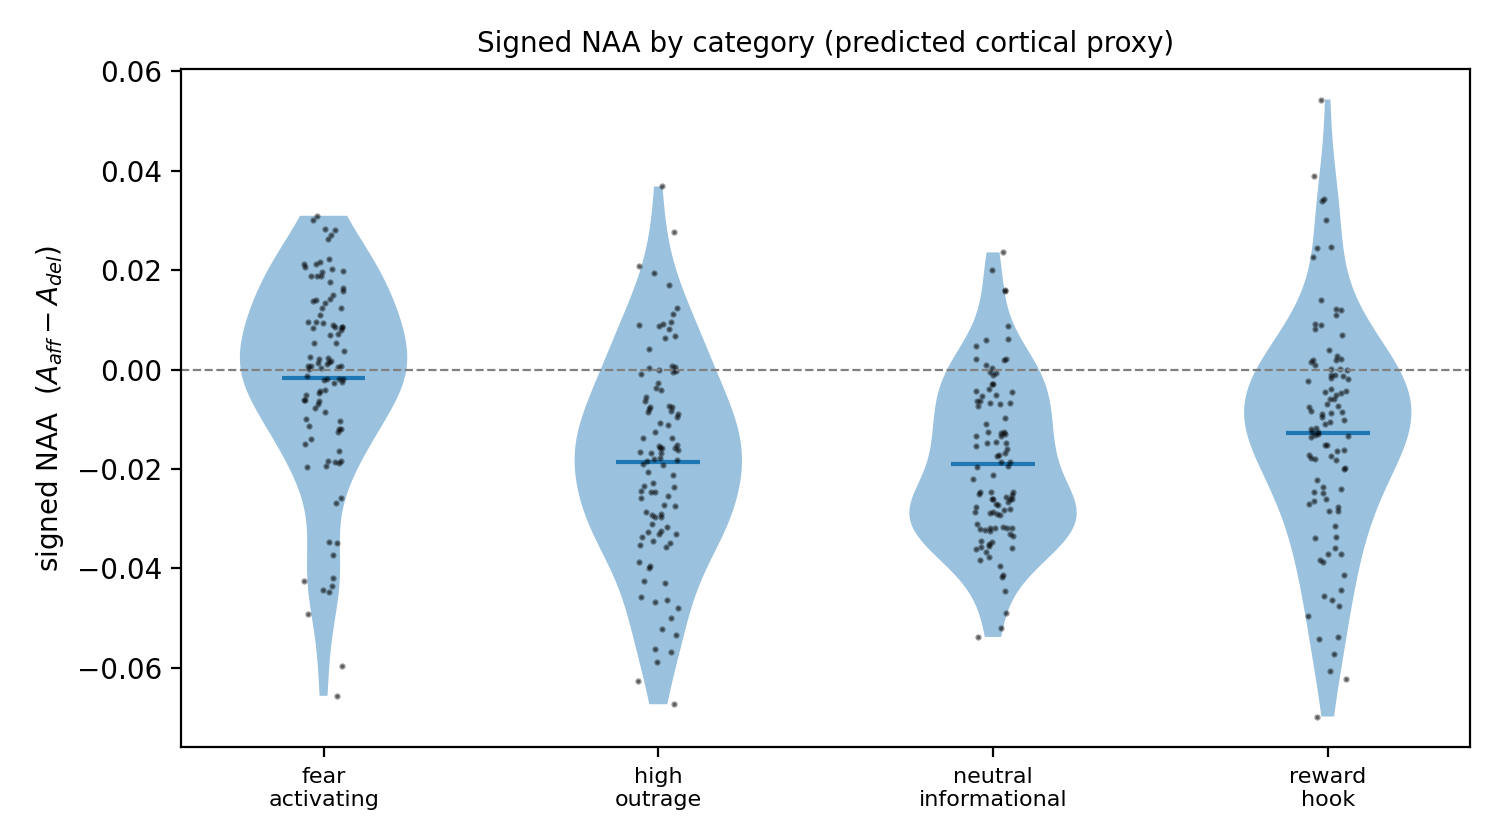
\includegraphics[width=0.9\textwidth]{../../services/inference/data/final/report/fig_violin.png}
\caption{Distribution of the signed index by category over all 400 items.}
\label{fig:violin}
\end{figure}

\begin{figure}[htbp]
\centering
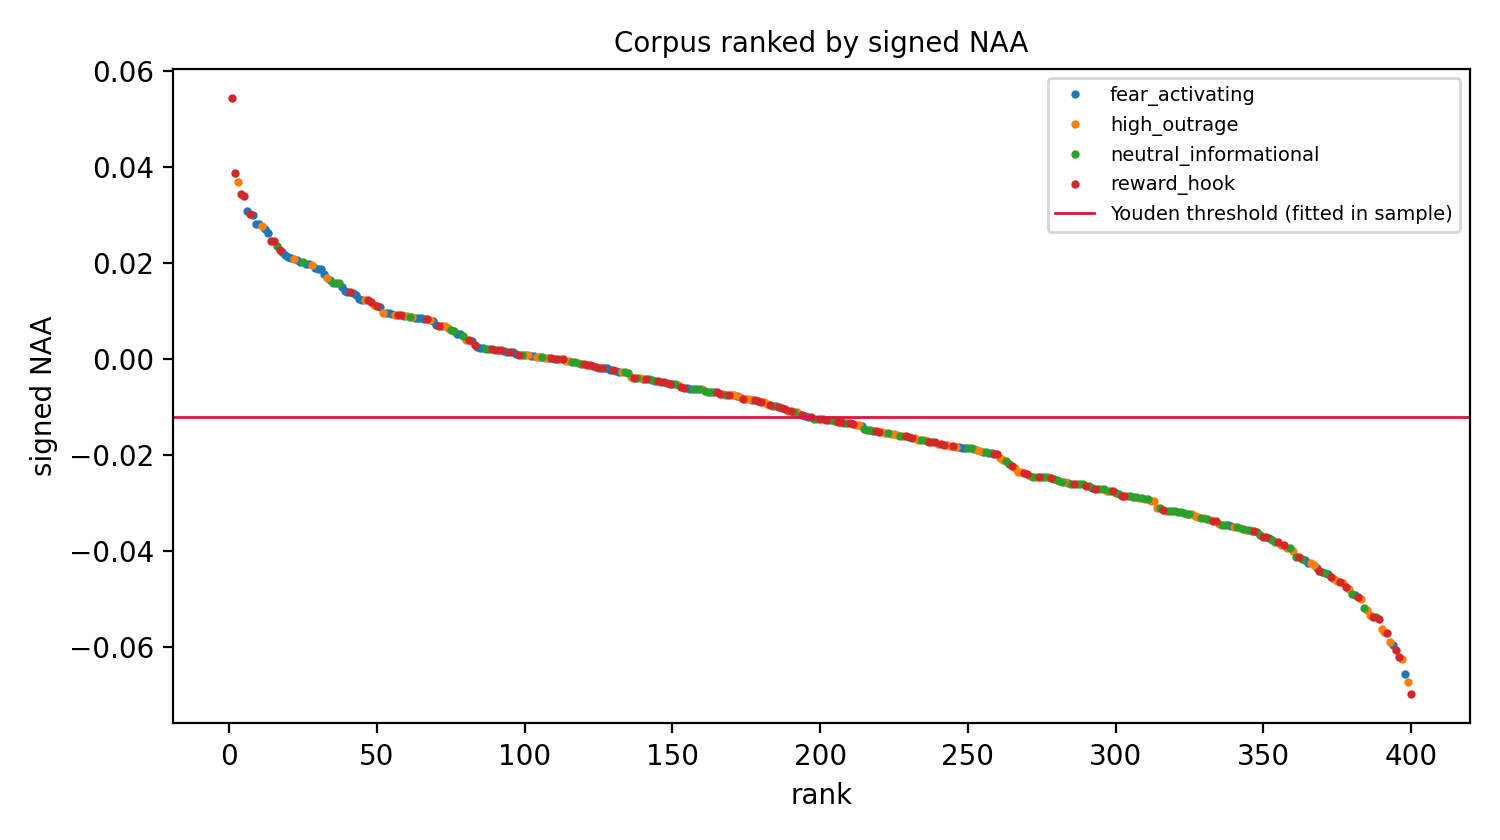
\includegraphics[width=0.9\textwidth]{../../services/inference/data/final/report/fig_ranked.png}
\caption{Every item ranked by the signed index, coloured by category.}
\label{fig:ranked}
\end{figure}

\subsection{The two components, taken separately}
\label{sec:components}

The signed index is a difference, and a difference discards information the corpus already
holds. $A_{\mathrm{aff}}$ and $A_{\mathrm{del}}$ are recorded per item, so each can be compared
against the neutral baseline on its own. This matters for high outrage in particular, where a
large symmetric response and no response are indistinguishable in a difference.

\begin{table}[htbp]
\centering
\begin{tabular}{@{}lrrr@{}}
\toprule
\textbf{Category} & $A_{\mathrm{aff}}$ & $A_{\mathrm{del}}$ & \textbf{signed} \\
\midrule
Fear activating       & $0.03206$ & $0.03385$ & $-0.00179$ \\
High outrage          & $0.02869$ & $0.04719$ & $-0.01850$ \\
Neutral informational & $0.01699$ & $0.03605$ & $-0.01906$ \\
Reward hook           & $0.02310$ & $0.03585$ & $-0.01275$ \\
\bottomrule
\end{tabular}
\caption{Category means of each component and of their difference, over all 400 items.}
\label{tab:components}
\end{table}

\begin{table}[htbp]
\centering
\begin{tabular}{@{}llrrr@{}}
\toprule
\textbf{Category vs neutral} & \textbf{Component} & \textbf{t} & \textbf{p} & \textbf{Cohen's d} \\
\midrule
Fear activating & $A_{\mathrm{aff}}$ & $+4.333$ & $2.365\times 10^{-5}$  & $+0.613$ \\
Fear activating & $A_{\mathrm{del}}$ & $-0.696$ & $4.875\times 10^{-1}$  & $-0.098$ \\
Fear activating & signed             & $+6.639$ & $3.283\times 10^{-10}$ & $+0.939$ \\
\midrule
High outrage    & $A_{\mathrm{aff}}$ & $+3.584$ & $4.263\times 10^{-4}$  & $+0.507$ \\
High outrage    & $A_{\mathrm{del}}$ & $+3.468$ & $6.521\times 10^{-4}$  & $+0.491$ \\
High outrage    & signed             & $+0.212$ & $8.320\times 10^{-1}$  & $+0.030$ \\
\midrule
Reward hook     & $A_{\mathrm{aff}}$ & $+1.842$ & $6.691\times 10^{-2}$  & $+0.261$ \\
Reward hook     & $A_{\mathrm{del}}$ & $-0.063$ & $9.501\times 10^{-1}$  & $-0.009$ \\
Reward hook     & signed             & $+2.254$ & $2.539\times 10^{-2}$  & $+0.319$ \\
\bottomrule
\end{tabular}
\caption{Welch comparisons of each component against neutral informational. High outrage moves both components by nearly the same amount and the difference between them by nothing; fear-activating content moves one component only.}
\label{tab:component-welch}
\end{table}

\textbf{High outrage is not a null in the components.} It raises $A_{\mathrm{aff}}$ by
$d = +0.507$ and $A_{\mathrm{del}}$ by $d = +0.491$, both at $p < 10^{-3}$, and it moves the
difference between them by $d = +0.030$ at $p = 0.832$. The two effects sit within four
hundredths of a standard deviation of each other. The category that fails to separate on the
index is the category that moves both networks together.

Fear-activating content behaves differently in exactly the way that reading predicts. It
raises $A_{\mathrm{aff}}$ by $d = +0.613$ and leaves $A_{\mathrm{del}}$ where it was
($d = -0.098$, $p = 0.488$), so the whole of its $d = +0.939$ on the index is a one-sided
movement. Reward-hook content sits between the two, with a small one-sided lift that does not
reach significance on its component alone.

The pattern holds at the level of the whole design. A one-way analysis of variance on each
component separately gives $F = 7.451$, $p = 7.276\times 10^{-5}$ for $A_{\mathrm{aff}}$ and
$F = 6.399$, $p = 3.052\times 10^{-4}$ for $A_{\mathrm{del}}$, against $F = 15.779$,
$p = 1.035\times 10^{-9}$ for the difference. Both components vary by category; the difference
varies more, because for two of the four categories one component moves while the other holds
still.

\begin{figure}[htbp]
\centering
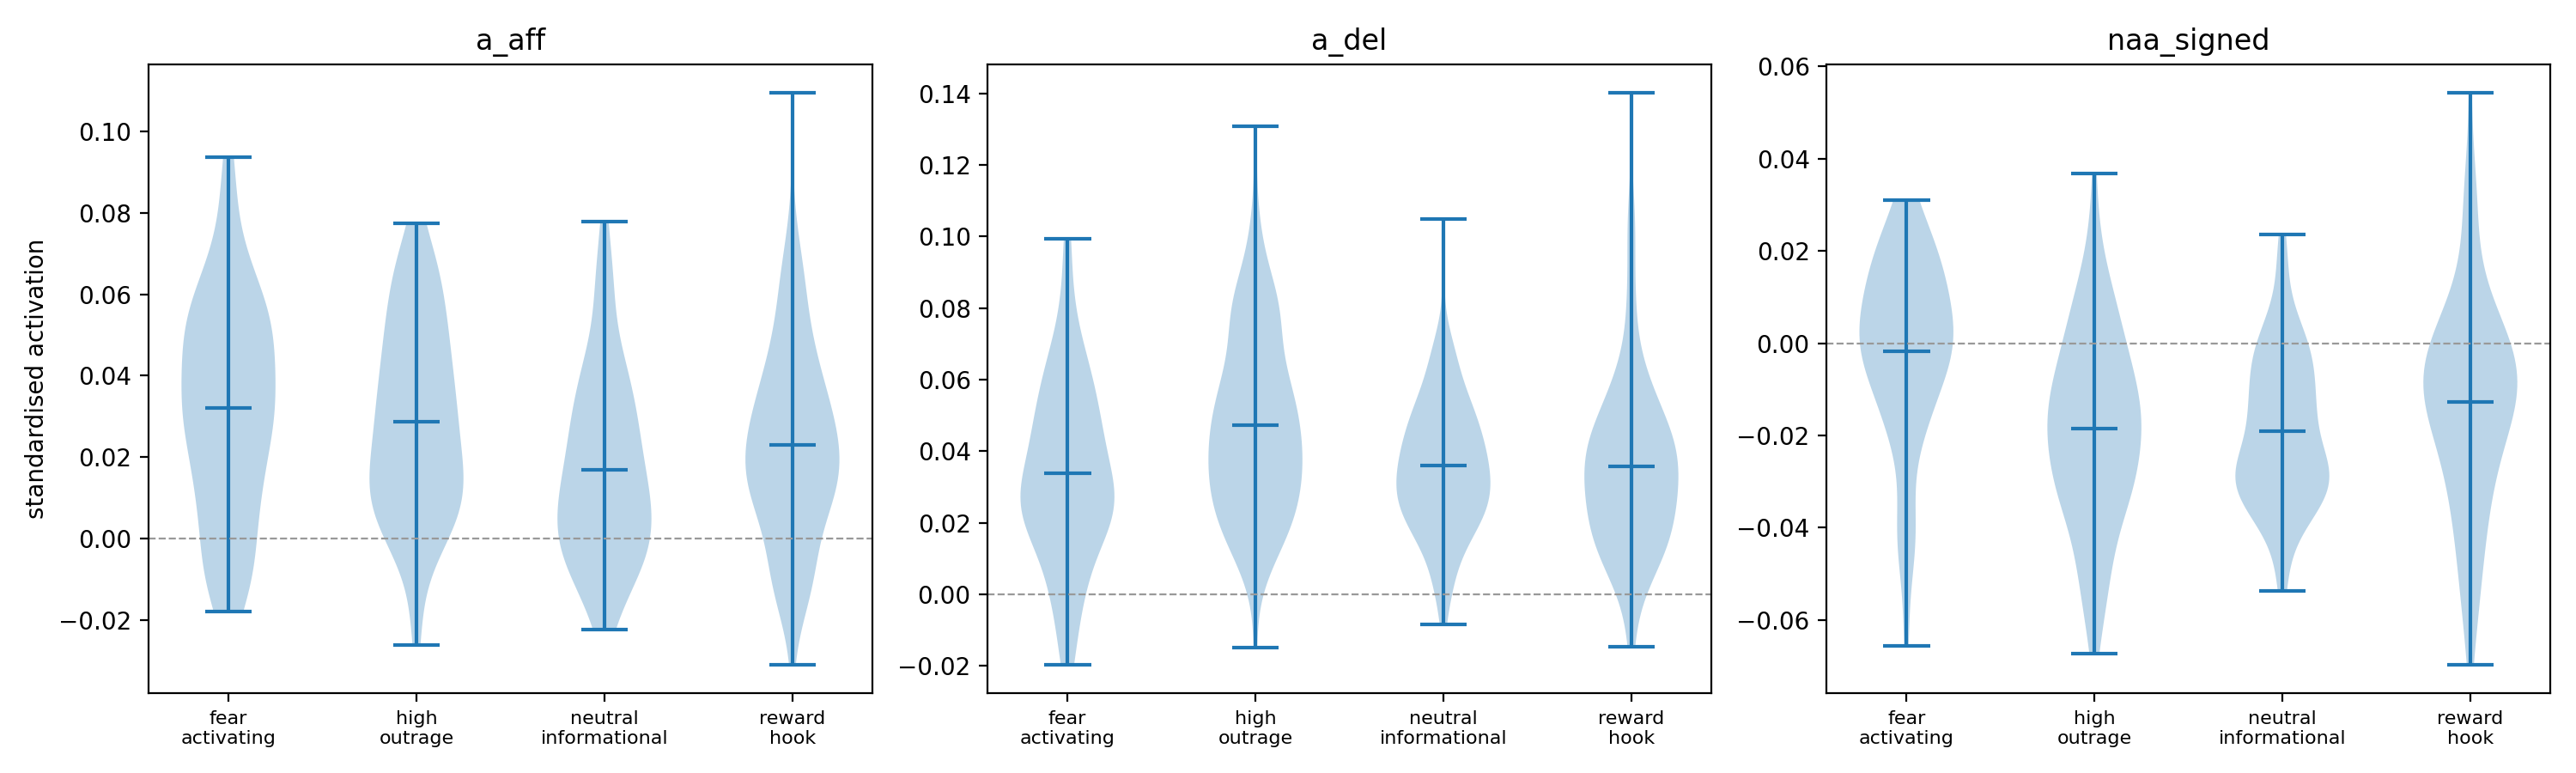
\includegraphics[width=0.95\textwidth]{../../services/inference/data/final/report/fig_components.png}
\caption{$A_{\mathrm{aff}}$, $A_{\mathrm{del}}$ and their signed difference by category over all 400 items. High outrage is elevated on both components and flat on the difference.}
\label{fig:components}
\end{figure}

This does not resolve the confound below, and it says nothing about whether the encoder tracks
cortex. What it does is remove one of the three readings of the outrage null from the list of
things this design cannot distinguish, which \S\ref{sec:outrage} takes up.

\subsection{The confound, stated before the interpretation}
\label{sec:confound}

Each category is drawn from exactly one source dataset: fear-activating from ISOT-fake, high
outrage from SemEval-2019 Task~4, reward-hook from Webis-Clickbait-17, and neutral from
PubMed and ISOT-true in equal parts. Category and provenance are therefore confounded by
construction, and the separation reported above is a separation \emph{between corpora}. It
cannot be attributed to framing rather than to the writing conventions, vocabulary and
editorial process of the source.

Length is not the confounding variable. Word counts are matched across categories at $167.4$,
$163.5$, $163.7$ and $162.2$ with standard deviations near $11$, which the corpus design
achieved deliberately. Provenance is the variable that was not controlled.

One piece of internal evidence argues against a pure source artifact. High outrage is drawn
from its own distinct source and does not separate from neutral on the index. An effect driven
only by provenance would be expected to move every category away from the baseline, not three
of four in an ordered way. The evidence is weaker than that sentence alone suggests:
\S\ref{sec:components} shows high outrage moving on both components and only the difference
staying flat, so a provenance effect is excluded only if it is assumed to act on one ROI union
at a time. This is suggestive, not decisive.

The design that would settle it is a corpus in which framing varies within a single source,
or in which one source appears in more than one category. Neither exists here, so the
attribution remains open and is carried into the discussion as a limitation rather than
resolved by argument.

\begin{figure}[htbp]
\centering
\includegraphics[width=0.95\textwidth]{../../services/inference/data/figures/B3_per_vertex_fear_activating-0000.pdf}
\caption{Predicted response for one fear-activating item at every one of the $20{,}484$
cortical vertices, on the pial surface. Vertices below the map's 70th percentile are left
unpainted so the anatomy remains readable; the threshold is stated in the figure. This is the
encoder's own output and not a smoothed or interpolated field.}
\label{fig:roi-means}
\end{figure}

\section{RQ III: phase structure and the coupling}
\label{sec:rq3}

The mean-field treatment of Chapter~3 gives the free energy $F(m) = a m^2 + b m^4 - hm$ with
$a = (1 - \beta J)/2$ and $b = 1/12$, coefficients derived from the self-consistency
condition rather than asserted. The phase structure is presented across a range of $\alpha$
and is not evaluated at a fitted value.

\subsection{The coupling is unidentified}

The calibration was run three times: on two partial corpora and on the completed 400 items.
On the partial runs the confidence interval comfortably included zero. On the full corpus it
does not, and the bootstrap over $10{,}000$ replicates places no mass below zero.

That is not a measurement of the coupling, for two reasons stated together because either
alone would be misleading. The fit's held-out $R^2$ is \textbf{negative}, so it predicts less
well than the sample mean on data it has not seen. And the estimate scales inversely with
$\beta J$, which no measurement in this study fixes: halving the assumed coupling strength
roughly doubles the fitted value. A single number would therefore report a choice of
$\beta J$ rather than a property of media.

The coupling is accordingly reported as unidentified, and no value is quoted.

\begin{figure}[htbp]
\centering
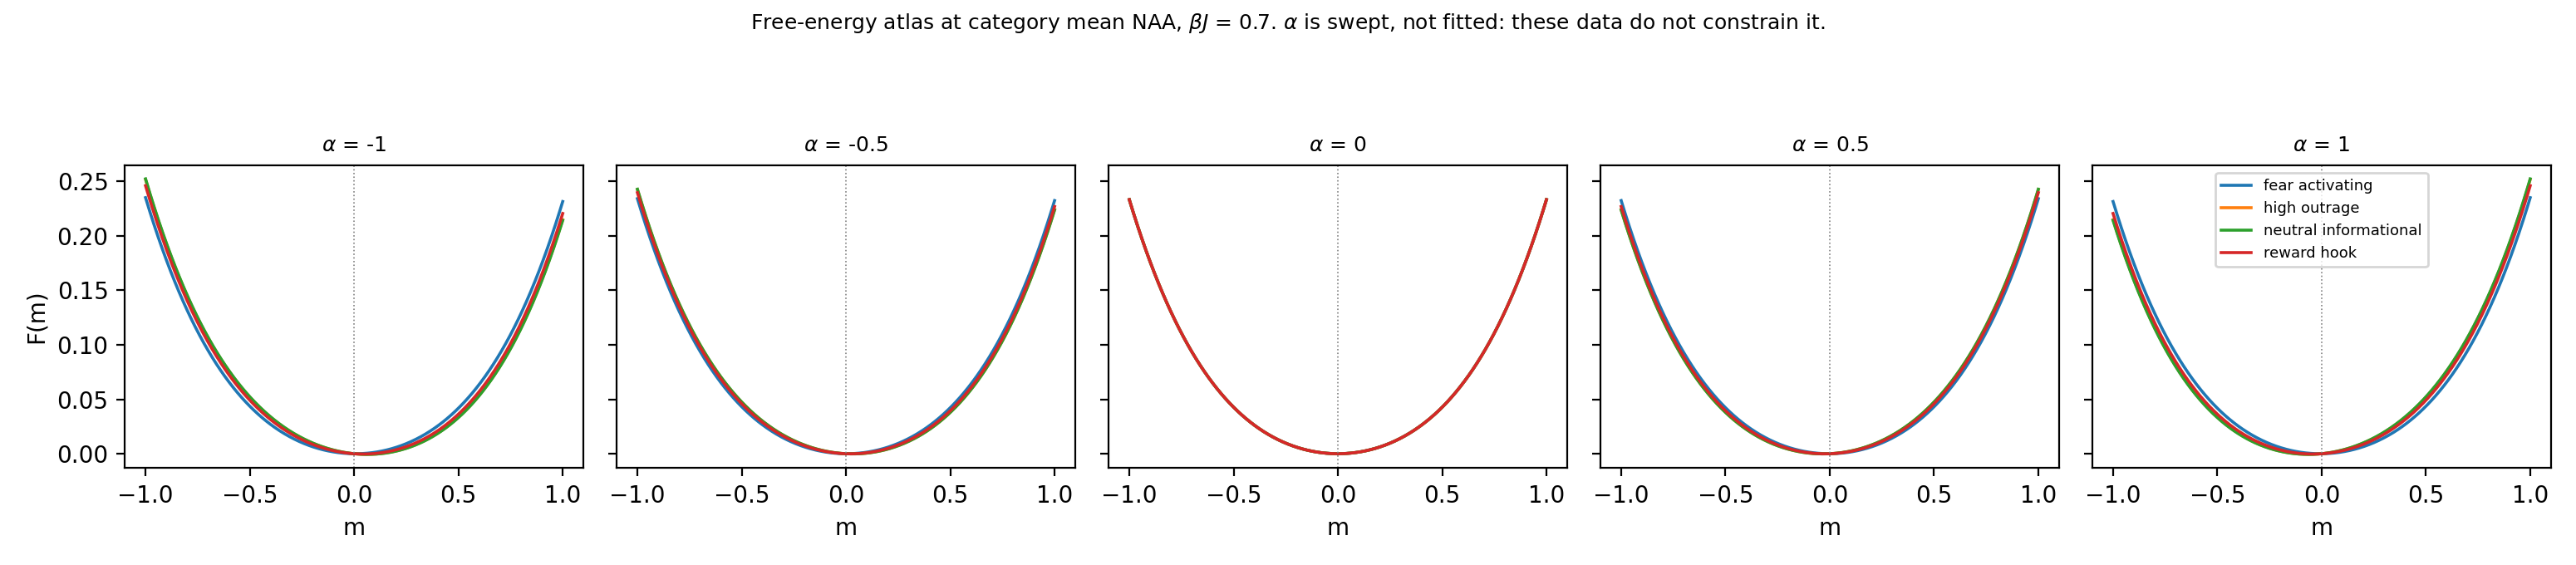
\includegraphics[width=0.9\textwidth]{../../services/inference/data/final/report/fig_free_energy_atlas.png}
\caption{Free energy at each category's measured mean, swept over $\alpha$. The coupling is
swept and never fitted, and no value of $\hat{\alpha}$ is quoted.}
\label{fig:free-energy-atlas}
\end{figure}

\subsection{The bound}

What the corpus does supply is the observable's measured spread, $\Delta X = 0.1241$ over the
range $-0.0698$ to $+0.0543$. Chapter~3's bound,
\begin{equation}
\alpha \;\ge\; \frac{h_c(\beta J)}{\Delta X},
\end{equation}
converts that spread into a statement about what the coupling would have to be:

\begin{table}[htbp]
\centering
\begin{tabular}{@{}lrr@{}}
\toprule
$\beta J$ & $h_c(\beta J)$ & $\alpha$ required \\
\midrule
$1.102$ & $0.02101$ & $0.1693$ \\
$1.496$ & $0.20541$ & $1.6553$ \\
$2.000$ & $0.53284$ & $4.2938$ \\
\bottomrule
\end{tabular}
\caption{The field bound at three values of the reduced coupling. The measured spread $\Delta X = 0.1241$ converts each critical field into the coupling any proposal of this mechanism would require.}
\label{tab:field-bound}
\end{table}

This is a necessary condition and not a sufficient one. Clearing it would not establish that
media of this measured spread moves populations; falling below it excludes the mechanism
within the model's assumptions. The value of the bound is that it requires no fit: it uses
the measured spread and the model's own spinodal, and it applies to any candidate observable
proposed as a field.

\section{Statistical power}
\label{sec:power}

The design's sensitivity was computed before the corpus was analysed and is reported
alongside every result above, so that a reader can see what this study could and could not
have found. At $\alpha = 0.05$ and $80\%$ power, with four categories of 100 and 300 against
100 for the classifier:

\begin{table}[htbp]
\centering
\begin{tabular}{@{}lr@{}}
\toprule
\textbf{Smallest detectable effect} & \textbf{Value} \\
\midrule
Category separation, $\eta^2$ & $0.0268$ \\
Equivalently, Cohen's $f$      & $0.1659$ \\
Classifier AUC                 & $0.5916$ \\
Equivalent separation $d$      & $0.3277$ \\
\bottomrule
\end{tabular}
\caption{Smallest effects this design could detect at $\alpha = 0.05$ and power $0.80$, fixed before the corpus was analysed.}
\label{tab:power}
\end{table}

Both observed effects clear these thresholds, and power at the observed values is $1.0$ for
the separation and $0.961$ for the AUC. Had either fallen below, the correct reading would
have been that the design could not have detected an effect of that size, not that no effect
exists.

\section{RQ IV: out of scope}

Research Question IV asked for per-modality mutual information across text, audio and video.
The amendment reduced the corpus to 400 text items and dropped the audio and video arms, so
the question as posed cannot be answered by this study. The narrowed text-only version was
not reached within the project timeline. It is recorded here as out of scope rather than
attempted and reported thinly.

\section{Summary of the answers}

\begin{enumerate}
\item \textbf{RQ I.} The ratio form of the index is undefined for $17.25\%$ of real content
and is replaced by the signed difference. Against the pre-scan dataset-derived label the index achieves
AUC $0.6274$, above the detectable floor and in the predicted direction, but modest. A TF-IDF
baseline on the same rows reaches $0.9758$, so the index is not the better detector; a
sentiment baseline does not clear chance.

\item \textbf{RQ II.} The four categories separate, $F = 15.779$, $p = 1.035 \times 10^{-9}$,
$\eta^2 = 0.1068$. The effect is concentrated in fear-activating content
($d = +0.939$); high outrage does not separate on the index at all, but raises both component
activations by almost the same amount ($d = +0.507$ and $d = +0.491$), so its flat difference is a
symmetric response rather than an absence of one. Category is confounded with source dataset,
so the separation cannot be attributed to framing.

\item \textbf{RQ III.} The coupling is unidentified and no value is quoted. The measured
spread $\Delta X = 0.1241$ yields a lower bound on any coupling capable of driving a
transition, reaching $\alpha \ge 4.2938$ at $\beta J = 2$.

\item \textbf{RQ IV.} Out of scope under the amendment.
\end{enumerate}

Every category mean remains negative throughout. Whatever the categories differ in, none of
them shows the affective-salience network leading in absolute terms.

\chapter{Discussion}
\label{ch:discussion}

Chapter~5 reported that the four categories separate, that the separation is carried almost
entirely by one of them, and that category is confounded with source dataset by construction.
This chapter asks what can be concluded from that, and is organised around the order in which
an examiner is entitled to doubt it.

\section{What the separation can and cannot support}

The measured effect, $\eta^2 = 0.1068$ at $p = 1.035\times10^{-9}$, is four times the
smallest effect the design could detect. Taken on its own terms it is unambiguous: the index
assigns systematically different values to the four groups of documents.

What it does not support is the sentence the proposal was written to test. Because each
category is drawn from a single source dataset (\S\ref{sec:confound}), a separation between
categories and a separation between corpora are the same measurement here. Fear-activating
items are ISOT-fake items. Whatever distinguishes ISOT-fake from PubMed and ISOT-true --- its
framing, but equally its vocabulary, its house style, its editorial process, its era --- is
folded into the effect and cannot be separated from it by any analysis of this data.

This is a design limitation, not an analytical one. No amount of statistical work on 400
items assembled this way can attribute the difference to framing.

\subsection{The evidence that argues against a pure source artifact}

Three observations bear on it, none decisive.

First, high outrage does not separate ($d = +0.030$, $p = 0.832$) despite coming from its own
distinct source, SemEval-2019 Task~4. If the index were simply detecting provenance, every
category drawn from a different corpus should move away from the baseline. Three of four
moving, in an ordered way, is a weaker pattern than pure source detection predicts.

Second, length is controlled. Word counts sit at $167.4$, $163.5$, $163.7$ and $162.2$ with
standard deviations near $11$. The most obvious surface confound was designed out.

Third, the ordering is not arbitrary with respect to the hypothesis. Fear-activating content
sits furthest from neutral and reward-hook content sits between. A source artifact carries no
reason to order itself along the dimension the study proposed.

Against these stands the plain fact that the confound exists and is complete. The honest
position is that the result is consistent with the hypothesis and equally consistent with a
corpus artifact, and that this study cannot choose between them.

\subsection{The experiment that would decide it}

The confound is removable by design, not by analysis. Two routes are available to a
successor:

\begin{enumerate}
\item \textbf{Within-source variation.} Draw all four categories from a single source, so
provenance is held constant while framing varies. Feasible where a source contains both
plainly-reported and emotively-framed material.
\item \textbf{Crossed design.} Ensure each source appears in more than one category, making
source and category statistically separable so their contributions can be estimated
independently.
\end{enumerate}

Either would convert the present result from a suggestive to an interpretable one. Neither
requires new instrumentation; both require rebuilding the corpus.

\section{Why high outrage does not separate}

The proposal expected outrage to separate most strongly, and it separated least. Three
readings deserve stating.

The first is that it is correct. Outrage framing may engage deliberative and affective
systems in more balanced measure than threat framing does, in which case a signed difference
between the two networks is precisely the wrong instrument for detecting it: a large
symmetric response and no response are indistinguishable in a difference.

The second is a property of the source. SemEval-2019 Task~4 labels hyperpartisan publishing
at the article level. Hyperpartisan is not synonymous with outrage-framed, and a corpus
selected on partisanship may contain a substantial fraction of items that are simply
argumentative rather than emotionally charged.

The third is the encoder. TRIBE was trained on naturalistic film and podcast viewing, and is
being asked to predict responses to synthesised speech from news text. There is no reason to
expect its sensitivity to be uniform across framing styles that were absent from training.

These are not ranked, because the data does not rank them.

\section{The instrument's standing}
\label{sec:standing}

Every value in this thesis is a prediction from a released encoder. No participant was
scanned, no brain was measured, and the observable is a cortical proxy computed from
predicted activation over two ROI unions.

That distinction is load-bearing here in a way it was not when the result looked like a null.
A null in predicted activation is a weak statement whichever way the encoder behaves. A
\emph{detected separation} in predicted activation is only a statement about media if the
encoder tracks cortex at all. The result reported in Chapter~5 therefore raises the stakes on
a question this study cannot answer from its own data.

\subsection{The checkpoint problem}

The released checkpoint is loaded in its average-subject configuration, which
\texttt{tribev2/demo\_utils.py} forces at load time. A commercial laboratory has published an
audit of that configuration reporting vertex-level $r = -0.0145$ against a measured
inter-subject ceiling of $+0.0508$: anti-correlated with real cortex, across four subjects
and all seven Yeo networks.

That audit is self-published by a company selling the per-subject alternative, uses four
subjects and one stimulus, and reports magnitudes near $0.015$ in either direction. It is a
claim about sign, not about effect size, and it has not been independently replicated. It
should not be accepted uncritically, and it cannot be dismissed either.

Work toward replicating it was begun within this project. Using the publicly released
Algonauts~2025 responses, the leave-one-subject-out noise ceiling was measured directly from
four subjects over all 1000 Schaefer parcels of episode \texttt{s01e01a}, 592 timepoints:
\begin{equation}
r_{\text{ceiling}} = 0.1517, \qquad 95\%\ \text{CI}\ [0.1484,\ 0.1551].
\end{equation}
An earlier figure of $0.2247$ is withdrawn. It was produced by a notebook cell that selected
the first key in the response file, which is a different episode from the one under
prediction, and whose orientation test could not fire on an array with fewer timepoints than
parcels, so the correlation ran across the parcel axis and the reported count of 482
``parcels'' was in fact the number of timepoints. The measurement now lives in a script that
takes the episode as an argument and asserts orientation against the atlas size.
This is the quantity any encoder must be judged against, and it is measured here rather than
quoted. It is larger than the audit's $+0.0508$ by construction and not by disagreement:
averaging vertices within a parcel cancels independent noise and raises correlations, so a
parcel-level ceiling and a vertex-level ceiling are not comparable numbers. The comparison
against the checkpoint's own predictions was not completed within this project's timeline and
is stated as unfinished rather than estimated.

\subsection{What this means for building on foundation models}

A technical report describing an architecture is not a warranty about the weights that are
released under its name. The checkpoint used here is cortical-only, which the proposal did
not anticipate; it is loaded in a configuration the accompanying paper does not foreground;
and its agreement with real cortex is contested in the literature. None of that is visible
from the paper.

The practical lesson generalises beyond this project: anyone building a measurement on a
released model should verify the checkpoint's properties from the artifact itself, as
\texttt{scripts/verify\_tribe\_checkpoint.py} does here, rather than inheriting them from the
publication.

\section{The coupling, and what the bound does instead}

The coupling between the index and the physics model's field is unidentified
(\S\ref{sec:rq3}): significant in sample, negative in held-out $R^2$, and inversely dependent
on a $\beta J$ that nothing in this study measures. Reporting a value would report a choice.

The bound is what survives. Because it requires only the observable's measured spread and the
model's own spinodal, $\alpha \ge h_c(\beta J)/\Delta X$ converts $\Delta X = 0.1241$ into a
statement no fit is needed to make: a coupling below $4.2938$ at $\beta J = 2$ cannot drive
the transition regardless of how the calibration is performed. This inverts the usual
practice in the sociophysics literature, where the field is assigned and the population is
shown to tip, without establishing that any real influence reaches the assigned magnitude.

That inversion is the contribution most likely to be reusable by others, because it applies
to any proposed field observable and can be evaluated before a corpus is collected.

\section{Session reliability, and what it permits}
\label{sec:reliability}

A second GPU session scanned 375 of the 400 items with identical text, identical code and
identical ROI definitions. That pair is a test-retest measurement, and it is reported here
because every effect in Chapter~5 otherwise rests on a single session with no statement of
how much of an item's score is the item and how much is the session.

Agreement between the two sessions, on the 375 items they share:

\begin{table}[htbp]
\centering
\begin{tabular}{lrrrr}
\hline
& $r$ & ICC(2,1) & $\mathrm{sd}(\Delta)$ & $\mathrm{sd}(\Delta)/\mathrm{sd}_{\text{between}}$ \\
\hline
$\mathrm{NAA}_{\text{signed}}$ & $0.8812$ & $0.8757$ & $0.01006$ & $0.475$ \\
$A_{\text{aff}}$ & $0.8768$ & $0.8696$ & $0.01210$ & $0.487$ \\
$A_{\text{del}}$ & $0.8575$ & $0.8544$ & $0.01285$ & $0.520$ \\
\hline
\end{tabular}
\caption{Agreement between the two scanning sessions over the 375 items both cover. ICC is reported beside $r$ because a session that shifted every score by a constant would still correlate perfectly.}
\label{tab:test-retest}
\end{table}

The intraclass correlation is reported alongside $r$ because a session that shifted every
score by a constant would still correlate perfectly, and a shift is precisely what a second
session can produce. The two agree closely here, so the disagreement is scatter rather than
offset.

\textbf{The separation replicates.} Recomputing the four-category ANOVA on the second session
over the same 375 items gives $\eta^2 = 0.0839$, $F = 11.328$, $p = 3.988\times10^{-7}$,
against $\eta^2 = 0.1054$, $F = 14.576$, $p = 5.397\times10^{-9}$ for the first session
restricted to those items. Both clear the smallest effect this design could detect,
$\eta^2 = 0.0268$. The separation reported in Chapter~5 is therefore not an artifact of one
session. The second session's effect is roughly a fifth smaller, which is the attenuation
that additional measurement error produces in a ratio of between-group to total variance.

\textbf{Per-item direction is not reliable.} The signed index is read as a direction, and
$49$ of $375$ items, $13.1\%$, reverse that direction between sessions. A statement that a
particular item is affective-leading is therefore not supportable by this instrument at this
precision, and none is made: no per-item verdict appears in the analysis, in the figures or
on the public interface. Group means over 100 items average this scatter down by an order of
magnitude, which is why the category-level result survives while the item-level one does not.

Both sessions are reported as measured. Neither is corrected toward the other and the two are
not averaged, because an average of two sessions would carry a precision that neither run
has.

\textbf{Scan order does not carry the separation.} The corpus took more than one session to
scan, which raises the question of whether position in the scan, and therefore session, is
doing the work attributed to category. It is not, and the reason is that items were scanned
interleaved rather than in category blocks: across thirds of the scan order the four
categories are balanced ($\chi^2 = 3.139$, $p = 0.7913$). There is a real drift, with mean
$\mathrm{NAA}_{\text{signed}}$ differing across thirds at $\eta^2 = 0.0167$, $p = 0.0353$.
Because it is orthogonal to category by construction, it adds scatter rather than bias:
removing the scan-third means before the category ANOVA moves the effect from
$\eta^2 = 0.1068$ to $\eta^2 = 0.1048$, $p = 1.588\times10^{-9}$. Had the corpus been scanned
one category at a time, this drift would have been indistinguishable from the finding.

\section{Limitations}

Stated here in full rather than distributed through the text.

\begin{enumerate}
\item \textbf{Category is confounded with source dataset.} The central limitation. Discussed
in \S\ref{sec:confound} and above.

\item \textbf{Single-session scores are noisy.} Test-retest ICC is $0.8757$ and the
session-to-session standard deviation is $47.5\%$ of the between-item standard deviation
(\S\ref{sec:reliability}). Category-level conclusions survive this; per-item ones do not.

\item \textbf{Predicted, not measured, activation.} No brain was scanned. Whether the
encoder tracks cortex is unresolved and contested.

\item \textbf{Cortical proxy, not a subcortical measurement.} The checkpoint is
cortical-only. The structures the original proposal named cannot be measured with it, and no
claim about them is made anywhere in this document.

\item \textbf{Average-subject configuration.} Forced by the loader. Whatever individual
variation the model can express is unavailable.

\item \textbf{Out-of-distribution stimuli.} The encoder was trained on naturalistic
audiovisual material and is fed synthesised speech from written text.

\item \textbf{The ratio form fails on $17.25\%$ of items}, and the reformulation to a signed
difference, while necessary, changes what the index means: it measures which network leads,
not by what proportion.

\item \textbf{English-language corpus from five specific sources, none of them Kenyan or
African.} A search for openly licensed Kenyan or African news data carrying usable labels
returned nothing suitable, so every item in the corpus originates from American or European
publishing. The measured spread is a property of that corpus, not of media in general, and
the bound inherits the limitation. Whether the instrument behaves the same way on media a
Kenyan reader actually encounters is untested, and assembling a labelled local corpus is the
most obvious extension of this work.

\item \textbf{Mean-field physics.} All-to-all coupling, one homogeneous population, a static
field, binary opinions. Network structure and heterogeneity generally lower $h_c$, so the
bound is conservative within the model and is not a universal statement.
\end{enumerate}

\section{What would be required next}

In order of what each would buy.

\textbf{A crossed or within-source corpus} would make the separation interpretable. It is the
cheapest of these and the one that most changes what can be claimed.

\textbf{Completing the validation} would establish whether the instrument measures anything
about brains. The noise ceiling is measured and the evaluation code is written and tested;
what remains is running the checkpoint over a held-out stimulus and correlating. It needs no
large compute.

\textbf{A subcortical checkpoint} would let the original proposal's question be asked as
posed. That means the training grid, the four source fMRI corpora and compute well outside
the scope of an undergraduate project, and it is recorded as future work rather than a plan.

\chapter{Conclusion}
\label{ch:conclusion}

\section{What was promised}

The proposal committed to an instrument. It said so three times: that the primary deliverable
is a functional Asynchronous Measurement Apparatus, that this is ``not a proposed future
application and not a conceptual description'', and that the project ``proposes a thermometer,
and delivers it as working, open-source code that can be run today''.

That framing governs how this work should be judged. A thermometer that reads a value nobody
expected is still a delivered thermometer. Failing to ship it would have been the failure.

\section{What was delivered}

\subsection{The apparatus}

The instrument exists and runs. Given a passage of text it synthesises speech, obtains word
timings, computes text and audio embeddings, passes them to the released encoder, and returns
a predicted response over $20{,}484$ cortical surface points, from which the index is
computed. It is open source, it is deployed, and it was run end to end over 400 items.

Its outputs are reproducible: the corpus file, the analysis scripts, the power calculation
and the physics all regenerate from the repository, and every number in Chapters~5 and~6 is
produced by a script rather than transcribed.

\subsection{The framework}

The mean-field treatment of Chapter~3 derives its Landau coefficients from the
self-consistency condition rather than asserting them, recovers the exact critical exponents
numerically as a check on the solver, and locates the spinodal field $h_c(\beta J)$ at which
bistability collapses.

From that follows the bound: for any observable $X$ proposed as a field through $h = \alpha
X$, no media-driven transition is possible unless
\begin{equation}
\alpha \;\ge\; \frac{h_c(\beta J)}{\Delta X}.
\end{equation}
This inverts the usual procedure in the sociophysics literature, where the field is assigned
by hand and the population is then shown to tip. It requires no fit, applies to any candidate
observable, and can be evaluated before a corpus is collected.

\subsection{The measurement}

All 400 items were scanned and verified. The four categories separate at $\eta^2 = 0.1068$,
$p = 1.035\times10^{-9}$, against a design powered to detect $0.0268$. Against the labels the
items carried before scanning, the index achieves AUC $0.6274$, above the detectable floor of
$0.5916$ and in the predicted direction.

The separation is carried almost entirely by fear-activating content ($d = +0.939$). High
outrage, the category the proposal expected to separate most, does not separate at all
($d = +0.030$, $p = 0.832$).

Every category mean is negative. The deliberative-control network is predicted to respond
more strongly than the affective-salience network for all four categories; they differ in how
far below zero they sit, not in which network leads.

\section{What is claimed, and what is not}

\textbf{Claimed.} That the instrument works and is reproducible. That the index assigns
systematically different values to these four groups of documents, at an effect size the
design was powered to detect, with the power statement reported alongside. That the measured
spread $\Delta X = 0.1241$ places a lower bound on any coupling capable of driving a
transition, reaching $\alpha \ge 4.2938$ at $\beta J = 2$.

\textbf{Not claimed.} That the index detects manipulation. That the separation is due to
framing rather than to source dataset: category and provenance are confounded by construction
and this design cannot distinguish them. That the coupling has been measured: it is
unidentified, and no value of $\hat{\alpha}$ appears anywhere in this document. That anything
here measures a brain: every value is a prediction from a released encoder, the observable is
a cortical proxy, and no participant was scanned.

The gap between those two lists is the honest content of this work.

\section{Contribution}

Three things, in the order they are likely to be useful to someone else.

\textbf{The bound.} A necessary condition on the coupling between any content observable and
an opinion-dynamics field, requiring only the observable's measured spread and the model's own
spinodal. It is the part of this work that transfers beyond the instrument that produced it.

\textbf{The instrument, with its limitation documented.} A working, open pipeline from text to
predicted cortical response, together with the finding that the released checkpoint is
cortical-only, that the loader forces its average-subject configuration, and that its
agreement with real cortex is contested. A technical report describing an architecture is not
a warranty about released weights, and this project's experience is a concrete instance of
that.

\textbf{The measurement and its confound.} A separation reported with the design's
sensitivity attached and its central weakness stated before its interpretation, together with
the specific experiment that would resolve it.

\section{Future work}

\textbf{Remove the confound.} A corpus in which framing varies within a single source, or in
which sources are crossed with categories, would make the separation interpretable. It needs
no new instrumentation, only a rebuilt corpus, and it is the single change that most alters
what can be claimed.

\textbf{Finish the validation.} Whether the encoder tracks cortex at all is unresolved and
determines what the measurement means. The noise ceiling has been measured directly from
public data at $0.1517$, CI $[0.1484,\ 0.1551]$, and the evaluation code is written and
tested. What remains is running the checkpoint over a held-out stimulus and correlating, which
needs no large compute.

\textbf{A subcortical checkpoint.} The structures the original proposal named cannot be
measured with a cortical-only model. Training one means the full grid, the source fMRI
corpora, and compute outside the scope of an undergraduate project.

\section{Code, data and the working instrument}

The pipeline, the corpus builder, the analysis scripts and the figure scripts are public at
\url{https://github.com/brn-mwai/monarch}. Every number in this document is written by a
named script into a JSON or CSV artifact and read from there rather than transcribed, so any
figure or table can be regenerated from the repository alone.

The instrument itself runs at \url{https://monarch.brianmwai.com}. It carries the complete
400-item corpus with each item's text, its pre-scan labels and its measured values, and it
draws the predicted response on the cortical surface for the items whose per-vertex maps were
kept. It answers questions about the corpus from a generated fact sheet and declines anything
the data does not cover, including any request for a coupling value.

\section{Closing}

This work set out to make an invisible property of media measurable, and to say honestly what
the measurement supports. It delivers a working instrument, a bound that constrains any future
proposal of this kind, and a result that is real, modest, and confounded in a way this
document states plainly rather than leaves to be discovered.

The physics is the part that survives whatever becomes of the encoder. Whether or not the
released checkpoint predicts any brain, the requirement that $\alpha \ge h_c(\beta J)/\Delta
X$ holds for every observable anyone proposes as a field, and the burden it places on such
proposals does not depend on this instrument being the right one.

The longer aim behind the project, set out in \S\ref{sec:phase1}, is a tool that a reader
rather than a researcher could use to ask whether something they are about to watch is built
to manipulate them or to hold their attention. This document is the first phase of that and
makes no claim to be more. It leaves an instrument, a characterised measurement, an honest
account of where that measurement fails, and a bound that does not depend on any of the
above. What it does not leave is a tool anyone should use to judge a particular article or
programme, and the four reasons why are measured in these chapters rather than guessed at.
Stating the destination is not the same as arriving at it, and the difference between them is
most of what this thesis reports.


% Shared by dissertation.tex and build_check.tex so the two cannot drift apart.
\begin{thebibliography}{9}
\addcontentsline{toc}{chapter}{References}
\bibitem{castellano2009} C.~Castellano, S.~Fortunato, V.~Loreto, Statistical physics of social dynamics, Rev. Mod. Phys. 81 (2009) 591--646. \href{https://doi.org/10.1103/RevModPhys.81.591}{doi:10.1103/RevModPhys.81.591}.
\bibitem{galam2008} S.~Galam, Sociophysics: A review of Galam models, Int. J. Mod. Phys. C 19 (2008) 409--440. \href{https://doi.org/10.1142/S0129183108012297}{doi:10.1142/S0129183108012297}.
\bibitem{sznajd2000} K.~Sznajd-Weron, J.~Sznajd, Opinion evolution in closed community, Int. J. Mod. Phys. C 11 (2000) 1157--1165. \href{https://doi.org/10.1142/S0129183100000936}{doi:10.1142/S0129183100000936}.
\bibitem{stauffer2008} D.~Stauffer, Social applications of two-dimensional Ising models, Am. J. Phys. 76 (2008) 470--473. \href{https://doi.org/10.1119/1.2779882}{doi:10.1119/1.2779882}.
\bibitem{mullick2025} P.~Mullick, P.~Sen, Sociophysics models inspired by the Ising model, Eur. Phys. J. B 98 (2025) 206. arXiv:2506.23837. \href{https://doi.org/10.1140/epjb/s10051-025-01053-7}{doi:10.1140/epjb/s10051-025-01053-7}.
\bibitem{crokidakis2012} N.~Crokidakis, Effects of mass media on opinion spreading in the Sznajd sociophysics model, Physica A 391 (2012) 1729. arXiv:1111.5750. \href{https://doi.org/10.1016/j.physa.2011.11.038}{doi:10.1016/j.physa.2011.11.038}.
\bibitem{azhari2023} Azhari, R.~Muslim, The external field effect on opinion formation based on the majority rule and the $q$-voter models on the complete graph, Int. J. Mod. Phys. C (2023) 2350088. arXiv:2305.06051. \href{https://doi.org/10.1142/S0129183123500882}{doi:10.1142/S0129183123500882}.
\bibitem{freitas2020} F.~Freitas, A.~R. Vieira, C.~Anteneodo, Imperfect bifurcations in opinion dynamics under external fields, J. Stat. Mech. (2020) 024002. \href{https://doi.org/10.1088/1742-5468/ab6848}{doi:10.1088/1742-5468/ab6848}.
\bibitem{sirbu2016} A.~S\^{i}rbu, V.~Loreto, V.~D.~P. Servedio, F.~Tria, Opinion dynamics: models, extensions and external effects, in: Participatory Sensing, Opinions and Collective Awareness, Springer, 2016, pp. 363--401. arXiv:1605.06326. \href{https://doi.org/10.1007/978-3-319-25658-0_17}{doi:10.1007/978-3-319-25658-0\_17}.
\bibitem{korbel2026} J.~Korbel, R.~Dahdoul, S.~Thurner, Empirical validation of the polarization transition in a double-random field model of elections, Phys. Rev. Lett. 136 (2026) 127402. arXiv:2510.00612. \href{https://doi.org/10.1103/9gjj-1df6}{doi:10.1103/9gjj-1df6}.
\bibitem{tribe2025} S.~d'Ascoli, J.~Rapin, Y.~Benchetrit, H.~Banville, J.-R.~King, TRIBE: TRImodal Brain Encoder for whole-brain fMRI response prediction, \href{https://arxiv.org/abs/2507.22229}{arXiv:2507.22229} (2025).
\bibitem{tribe2026} S.~d'Ascoli, J.~Rapin, Y.~Benchetrit, T.~Brooks, K.~Begany, J.~Raugel, H.~Banville, J.-R.~King, A foundation model of vision, audition, and language for in-silico neuroscience, \href{https://arxiv.org/abs/2605.04326}{arXiv:2605.04326} (2026).
\bibitem{goldenfeld1992} N.~Goldenfeld, Lectures on Phase Transitions and the Renormalization Group, Addison-Wesley, 1992; reprinted CRC Press, 2018. \href{https://doi.org/10.1201/9780429493492}{doi:10.1201/9780429493492}.
\bibitem{ahmed2017} H.~Ahmed, I.~Traore, S.~Saad, Detection of online fake news using n-gram analysis and machine learning techniques, in: Intelligent, Secure, and Dependable Systems in Distributed and Cloud Environments (ISDDC 2017), Lecture Notes in Computer Science 10618, Springer, 2017, pp. 127--138. \href{https://doi.org/10.1007/978-3-319-69155-8_9}{doi:10.1007/978-3-319-69155-8\_9}.
\bibitem{kiesel2019} J.~Kiesel, M.~Mestre, R.~Shukla, E.~Vincent, P.~Adineh, D.~Corney, B.~Stein, M.~Potthast, SemEval-2019 Task 4: Hyperpartisan news detection, in: Proceedings of the 13th International Workshop on Semantic Evaluation, 2019, pp. 829--839. \href{https://doi.org/10.18653/v1/S19-2145}{doi:10.18653/v1/S19-2145}.
\bibitem{potthast2018} M.~Potthast, T.~Gollub, K.~Komlossy, S.~Schuster, M.~Wiegmann, E.~P. Garces Fernandez, M.~Hagen, B.~Stein, Crowdsourcing a large corpus of clickbait on Twitter, in: Proceedings of the 27th International Conference on Computational Linguistics (COLING), 2018, pp. 1498--1507. \url{https://aclanthology.org/C18-1127/}.
\bibitem{pubmed} National Center for Biotechnology Information, PubMed, accessed through the Entrez Programming Utilities, \url{https://pubmed.ncbi.nlm.nih.gov}.
\bibitem{hutto2014} C.~J. Hutto, E.~Gilbert, VADER: A parsimonious rule-based model for sentiment analysis of social media text, in: Proceedings of the Eighth International AAAI Conference on Weblogs and Social Media (ICWSM), 2014, pp. 216--225. \href{https://doi.org/10.1609/icwsm.v8i1.14550}{doi:10.1609/icwsm.v8i1.14550}.
\bibitem{algonauts2025} A.~T. Gifford, D.~Bersch, M.~St-Laurent, et al., The Algonauts Project 2025 Challenge: How the human brain makes sense of multimodal movies, \href{https://arxiv.org/abs/2501.00504}{arXiv:2501.00504} (2025).
\bibitem{schaefer2018} A.~Schaefer, R.~Kong, E.~M. Gordon, T.~O. Laumann, X.-N. Zuo, A.~J. Holmes, S.~B. Eickhoff, B.~T.~T. Yeo, Local-global parcellation of the human cerebral cortex from intrinsic functional connectivity MRI, Cereb. Cortex 28 (2018) 3095--3114. \href{https://doi.org/10.1093/cercor/bhx179}{doi:10.1093/cercor/bhx179}.
\bibitem{yeo2011} B.~T.~T. Yeo et al., The organization of the human cerebral cortex estimated by intrinsic functional connectivity, J. Neurophysiol. 106 (2011) 1125--1165. \href{https://doi.org/10.1152/jn.00338.2011}{doi:10.1152/jn.00338.2011}.
\bibitem{sapient2026} The Sapient Company, The Faceless Brain, self-published technical report, 2026, \url{https://thesapientcompany.com/research}.
\end{thebibliography}


\end{document}
